\documentclass{vgtc}                          % final (conference style)

\ifpdf%                                % if we use pdflatex
  \pdfoutput=1\relax                   % create PDFs from pdfLaTeX
  \pdfcompresslevel=9                  % PDF Compression
  \pdfoptionpdfminorversion=7          % create PDF 1.7
  \ExecuteOptions{pdftex}
  \usepackage{graphicx}                % allow us to embed graphics files
  \DeclareGraphicsExtensions{.pdf,.png,.jpg,.jpeg} % for pdflatex we expect .pdf, .png, or .jpg files
\else%                                 % else we use pure latex
  \ExecuteOptions{dvips}
  \usepackage{graphicx}                % allow us to embed graphics files
  \DeclareGraphicsExtensions{.eps}     % for pure latex we expect eps files
\fi%

%% it is recomended to use ``\autoref{sec:bla}'' instead of ``Fig.~\ref{sec:bla}''
%\graphicspath{{figures/}{pictures/}{images/}{./}} % where to search for the images
 \usepackage[utf8]{inputenc}
 
\usepackage{microtype}                 % use micro-typography (slightly more compact, better to read)
\PassOptionsToPackage{warn}{textcomp}  % to address font issues with \textrightarrow
\usepackage{textcomp}                  % use better special symbols
\usepackage{mathptmx}                  % use matching math font
\usepackage{times}                     % we use Times as the main font
\renewcommand*\ttdefault{txtt}         % a nicer typewriter font
\usepackage{cite}                      % needed to automatically sort the references
\usepackage{tabu}                      % only used for the table example
\usepackage{booktabs}                  % only used for the table example

\onlineid{0}

\vgtccategory{Research}

\vgtcinsertpkg


\title{Learning PAC}

\author{Andres J. Montenegro Bello\thanks{e-mail: montenegroandresj@gmail.com}\\      \scriptsize GitHub : AndresJuniorMontenegro%
\and Raul Huaman Pajares \thanks{e-mail: rahuamanpa@gmail.com }\\ %
     \scriptsize GitHub : rhuamanpa\\
\and Repositorio \\
     \scriptsize https://github.com/rhuamanpa/Pac-Learning
}

%% Abstract section.
\abstract{ We will analize PAC learning, the type of uses that we can apply with PAC learning with machine learning and show some samples used by big companies like Facebook and Youtube to make incomes at the same time we will make a project using PAC learning using python that will recognize some facial gestures.%
} % end of abstract

%%%%%%%%%%%%%%%%%%%%%%%%%%%%%%%%%%%%%%%%%%%%%%%%%%%%%%%%%%%%%%%%
%%%%%%%%%%%%%%%%%%%%%% START OF THE PAPER %%%%%%%%%%%%%%%%%%%%%%
%%%%%%%%%%%%%%%%%%%%%%%%%%%%%%%%%%%%%%%%%%%%%%%%%%%%%%%%%%%%%%%%%

\begin{document}

\firstsection{Introduction}

\maketitle

%% \section{Introduction} %for journal use above \firstsection{..} instead
La probabilidad aproximada correcta (PAC), propuesta por L.Valiant,
es un marco de referencia estatico para aprender usar datos de entrenamiento.
\\
\\
En su forma mas simple y para un modelo tipico de tarea, la teoria
del aprendizaje PAC intentan relacionar, precision y confianza 
estadistica del modelo al numero de ejemplos de entrenamientos 
usados.
\\
\\
Uno de los conceptos más importantes en este sentido es medir la
complejidad de una clase de hipótesis $H$. En cualquier modelo de
aprendizaje automático, el objetivo final es encontrar una clase de
hipótesis que logre una alta precisión en el conjunto de
entrenamiento y que tenga un bajo error de generalización en el conjunto
de prueba. Para esto, requerimos que la clase de hipótesis $H$ se
aproxime al concepto de clase $C$ que determina las etiquetas para la
distribución $D$. Como tanto $C$ como $D$ son desconocidos, tratamos
de modelar $H$ en base al conjunto de muestras conocido $S$ y sus etiquetas.

\textbf{Generalizacion del error: }
El error de generalización de una hipótesis $h$ es la expectativa del
error en una muestra $x$ elegida de la distribución $D$.

\textbf{Error empirico: }
Esta es la media del error de la hipótesis $h$ en la muestra $S$ del 
tamaño $m$.

Habiendo definido el error de generalización y el error empírico de
esta manera, podemos establecer el objetivo del aprendizaje de la
siguiente manera.
\newline
\newline
\textit{El objetivo del aprendizaje es tener el error empírico
aproximado al error de generalización con alta probabilidad.}
\newline
\newline
Este tipo de marco de aprendizaje se conoce como Aprendizaje PAC
(Probablemente Aproximadamente Correcto). Formalmente, una clase de
concepto $C$ es $PAC-aprendible$ si hay algún algoritmo $A$ para el 
cual el error de generalización en una muestra $S$ derivado de la 
distribución $D$ es muy bajo (menor que $\epsilon$) con alta 
probabilidad (mayor que $1- \delta$). En otras palabras, podemos decir que para una
clase apta para PAC, la precisión es alta con buena confianza.
\\
\\
Se adjuntara una imagen en la cual dara una descripcion general del aprendizaje PAC.
\\
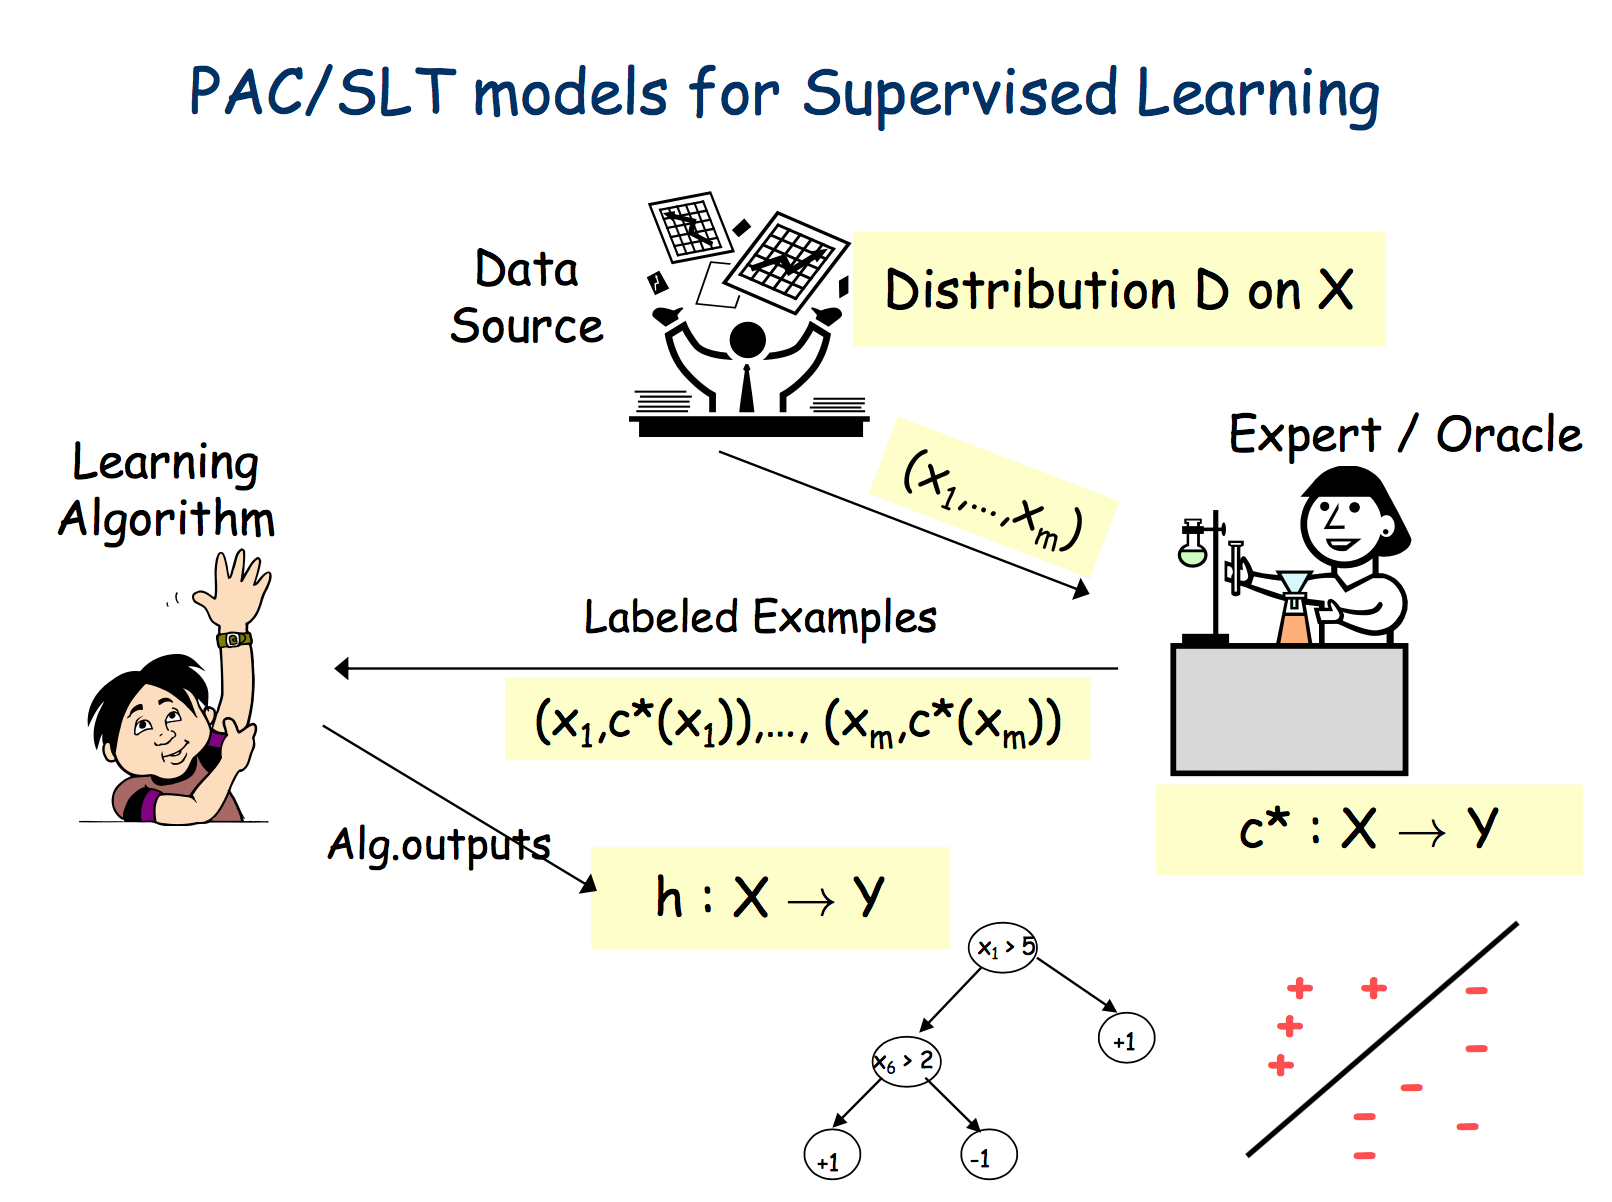
\includegraphics[scale=0.15]{pac.png} 
